\documentclass{sig-alternate-05-2015}
\usepackage[T1]{fontenc}
\usepackage[utf8]{inputenc}
\synctex=-1 
\usepackage[english]{babel}

\usepackage[hidelinks]{hyperref} % back-referencing + hyperlinks

\usepackage{xspace}
%\usepackage{subscript}
\usepackage{multirow}
\usepackage[font=small]{caption}
\captionsetup{skip=4pt}

\usepackage{subcaption}
\usepackage{graphicx}
\usepackage{comment}
\usepackage{tabularx}

\usepackage[normalem]{ulem}
\usepackage{fixltx2e}
\usepackage{booktabs}
\usepackage{pslatex}
%\usepackage{mathptmx,helvet,courier}
\usepackage[inline]{enumitem}
\usepackage{flushend}

\newcommand{\mytitle}{How the R Community Creates and Curates Knowledge:\\A Comparative Study of Stack Overflow and Mailing Lists}
\newcommand{\myauthor}{Carlos Arturo Gómez Teshima et al.}
\newcommand{\mysubject}{Interplay of multiple media channels}
\newcommand{\mykeywords}{Knowledge curation, Case study}

% PDF metadata. Disable when using latexdiff and enable for final version.
%\usepackage[unicode=true,
%            bookmarks=false,breaklinks=true,pdfborder={0 0 0},
%            backref=none,colorlinks=false]{hyperref}
\hypersetup{pdftitle={\mytitle},
             pdfauthor={\myauthor},
             pdfsubject={\mysubject},
             pdfkeywords={\mykeywords}
}


\newenvironment{packed_enum}{
\begin{enumerate}[itemsep=3pt, topsep=2pt, leftmargin=2.4em, parsep=0pt]
}{\end{enumerate}}

% Comments
% commands for inserting comments
\usepackage{color}
\usepackage{ifthen}
\newboolean{showcomments}
\setboolean{showcomments}{true} % toggle to show or hide comments
\ifthenelse{\boolean{showcomments}}
  {
		%\usepackage{showkeys} %Show lables and refs
		\newcommand{\nbb}[2]{
		% \fbox{\bfseries\sffamily\scriptsize#1}
		\fcolorbox{black}{yellow}{\bfseries\sffamily\scriptsize#1}
		{\sf$\blacktriangleright$\textcolor{blue}{\textit{#2}}$\blacktriangleleft$}
		% \marginpar{\fbox{\bfseries\sffamily#1}}
		}
        \newcommand{\dmg}[1]{{\color{blue}\emph{Daniel says: #1}}\xspace}
        \newcommand{\alexey}[1]{{\color{cyan}\emph{Alexey says: #1}}\xspace}
        \newcommand{\gpoo}[1]{{\color{red}\emph{Germán says: #1}}\xspace}
        \newcommand{\peggy}[1]{{\color{magenta}\emph{Peggy says: #1}}\xspace}
        \newcommand{\cassie}[1]{{\color{magenta}\emph{Cassie says: #1}}\xspace}
        \newcommand{\todo}[1]{\textcolor{red}{{\sc #1}}}
        \newcommand{\internalnote}[1]{\marginpar{\scriptsize note: #1}}
        \newcommand{\version}{\emph{\scriptsize{$-$\today$-$}}}
		\newcommand{\remarks}[1]{\color{red}[#1]\color{black}}
		\newcommand{\modified}[1]{\color{blue}[#1]\color{black}}
		\newcommand{\raw}{$\rightarrow$}
		\newcommand{\ins}[1]{\textcolor{blue}{\uline{#1}}} % please insert
		\newcommand{\del}[1]{\textcolor{red}{\sout{#1}}} % please delete
		\newcommand{\chg}[2]{\textcolor{red}{\sout{#1}}{\raw}\textcolor{blue}{\uline{#2}}} % please change
		\newcommand{\ugh}[1]{\textcolor{red}{\uwave{#1}}} % please rephrase
		\newcommand{\cn}{\textcolor{blue}{[citation needed]}\xspace}
  }
  {
        \newcommand{\dmg}[1]{}
        \newcommand{\gpoo}[1]{}
		\newcommand{\nbb}[2]{}
        \newcommand{\todo}[1]{}
        \newcommand{\internalnote}[1]{}
		\newcommand{\remarks}[1]{}
		\newcommand{\modified}[1]{#1}
		\newcommand{\version}{}
		\newcommand{\ugh}[1]{#1} % please rephrase
		\newcommand{\ins}[1]{#1} % please insert
		\newcommand{\del}[1]{} % please delete
		\newcommand{\chg}[2]{#2} % please change
		\newcommand{\cn}{}{}
  }

\newcommand{\channel}{communication channel\xspace}
\newcommand{\channels}{communication channels\xspace}
\newcommand{\Channel}{Communication channel\xspace}
\newcommand{\Channels}{Communication channels\xspace}

\newcommand{\SO}{Stack Overflow\xspace}
\newcommand{\RH}{R-help\xspace}

\newcommand{\rqa}{What types of knowledge are shared on Stack Overflow and the R-help mailing list within the R community?}
\newcommand{\rqb}{How is the knowledge constructed on Stack Overflow and the R-help mailing list?}
\newcommand{\rqc}{Why do certain users post to both Stack Overflow and the R-help mailing list?}
%\newcommand{\rqd}{What are the advantages and disadvantages of using Stack Overlow or the R-help mailing list?}

\newcommand{\reca}{Choose the correct channel}
\newcommand{\recb}{Be aware of the channel rules and the basic concepts and nomenclature used}
\newcommand{\recc}{Provide good background to the question}
\newcommand{\recd}{Learn to use external resources}
\newcommand{\rece}{Act altruistically}




%%% Local Variables:
%%% mode: latex
%%% TeX-master: "knowledge-curation.tex"
%%% End:


\begin{document}

% Copyright
\setcopyright{acmcopyright}
%\setcopyright{acmlicensed}
%\setcopyright{rightsretained}
%\setcopyright{usgov}
%\setcopyright{usgovmixed}
%\setcopyright{cagov}
%\setcopyright{cagovmixed}


% DOI
%\doi{10.475/123_4}

% ISBN
%\isbn{123-4567-24-567/08/06}

%Conference
\conferenceinfo{MSR '16}{May 14--15, 2016, Austin, TX, USA}

%\acmPrice{\$15.00}

%
% --- Author Metadata here ---
\conferenceinfo{MSR}{'16 Austin, Texas USA}
%\CopyrightYear{2007} % Allows default copyright year (20XX) to be over-ridden - IF NEED BE.
%\crdata{0-12345-67-8/90/01}  % Allows default copyright data (0-89791-88-6/97/05) to be over-ridden - IF NEED BE.
% --- End of Author Metadata ---

%
% General information
%


\title{\mytitle}

\numberofauthors{1}

\author{
  \alignauthor{Carlos Gómez Teshima, Alexey Zagalsky, Margaret-Anne Storey, Daniel M. German, Germán Poo-Caamaño\\
    \affaddr{University of Victoria}\\
    \affaddr{Victoria, BC, Canada}\\
    \email{\{teshima, alexeyza, mstorey, dmg, gpoo\}@uvic.ca}}\\
}

% \author{
%     \alignauthor
%     Carlos Gómez Teshima\\
%     \affaddr{University of Victoria}\\
%     \affaddr{Victoria, BC, Canada}\\
%     \email{teshima@uvic.ca}
%     \alignauthor 
%     Alexey Zagalsky\\
%     \affaddr{University of Victoria}\\
%     \affaddr{Victoria, BC, Canada}\\
%     \email{alexeyza@uvic.ca}
%     \and
%     \alignauthor
%     Margaret-Anne Storey\\
%     \affaddr{University of Victoria}\\
%     \affaddr{Victoria, BC, Canada}\\
%     \email{mstorey@uvic.ca}
%     \alignauthor 
%     Daniel M. German\\
%     \affaddr{University of Victoria}\\
%     \affaddr{Victoria, BC, Canada}\\
%     \email{dmg@uvic.ca}
%     \alignauthor
%     Germán Poo-Caamaño\\
%     \affaddr{University of Victoria}\\
%     \affaddr{Victoria, BC, Canada}\\
%     \email{gpoo@uvic.ca}
% }

\date{\the\year}

\maketitle

\begin{abstract}
One of the many effects of social media in software development is the flourishing of very large communities of practice where members share a common interest, such as programming languages, frameworks, and tools. These communities of practice use many different \channels and little is known about how these communities create, share, and curate knowledge using such channels.

In this paper, we report a qualitative study of how one community of practice---the R software development community---creates and curates knowledge associated with questions and answers (Q\&A) in two of its main \channels: the R-tag in Stack Overflow and the R-users mailing list. The results reveal that knowledge is created and curated in two main forms: participatory, where multiple members explicitly collaborate, and crowdsourced, where individuals mostly work independently of each other. The contribution of this paper is a characterization of the types of knowledge that are exchanged by these communities of practice, including a description of the reasons why members choose one channel over the other.  Finally, this paper enumerates a set of recommendations to assist practitioners in the use of multiple channels for Q\&A. 

%\alexey{I feel we can do better with the abstract, but only after we have the rest of the paper done.}
\end{abstract}

%
% The code below was generated with the tool at
% http://dl.acm.org/ccs.cfm
%
\begin{CCSXML}
<ccs2012>
<concept>
<concept_id>10003120.10003130.10003131.10003235</concept_id>
<concept_desc>Human-centered computing~Collaborative content creation</concept_desc>
<concept_significance>500</concept_significance>
</concept>
</ccs2012>
\end{CCSXML}

\ccsdesc[500]{Human-centered computing~Collaborative content creation}

%
% End generated code
%

%
%  Use this command to print the description
%
\printccsdesc

\keywords{\mykeywords}

% vim: set fenc=utf-8 ft=latex encoding=utf-8
% -*- mode: latex; coding: UTF-8; -*-
%!TEX root = knowledge-curation.tex
\section{Introduction}
\label{cha:introduction}
The adoption and emergence of socially enabled tools and channels (e.g., GitHub, \SO, mailing lists) has fostered the formation of large \textit{communities of practice} where members share a common interest, such as programming languages, frameworks, and tools~\cite{Storey2014}. These communities rely on and use many different communication channels, however, little is known about how they create, share, and curate knowledge using such channels. 

One prominent community of practice is the R community. The R programming language is an open source project without commercial backing that relies heavily on its rapidly growing and highly heterogeneous software development community. The R community plays an important role in the diffusion of the R language; members have numerous resources for learning the language and receiving help, such as mailing lists, blogs, books, online and offline courses, and question \& answer sites (e.g., \SO). While the R community benefits from this vast and rich corpus of knowledge, it also drives the creation and curation of the information.

Without a single entity directing and controlling it, the R language has grown organically from its community. Similar to other communities of practice, knowledge is exchanged and curated in many \channels, and two particular \channels are at the center of this process: the \textit{\RH mailing list} and \textit{\SO}. The \RH mailing list was created to assist those using the language, and while \SO is not specifically oriented towards R, its section dedicated to R (the R tag) has grown rapidly\footnote{\href{http://www.r-bloggers.com/r-is-the-fastest-growing-language-on-stackoverflow/}{http://www.r-bloggers.com/r-is-the-fastest-growing-language-on-stackoverflow/}}.

\SO has revolutionized the way programmers seek knowledge~\cite{li2013help,Vasilescu2014c}, assuming the role of a capable ``expert on call'' that is able---and willing---to answer questions of any level of difficulty about any programming technology (R included). \SO's gamification features guarantee that enthusiastic experts will answer questions, often within minutes of being posted~\cite{Mamykina2011}. Equally important is the ability of \SO's users to curate the knowledge being created, making sure that the best answers surface to the top and become a valuable asset to those seeking an answer now or in the future. \SO has become a popular and effective tool for creating, curating, and exchanging knowledge, including knowledge about the R language.

One would expect that the traffic in the \RH mailing list would begin to fizzle as \SO popularity increased. If \SO is so effective at matching those who seek knowledge with those that have it, doesn't that obviate most of the need for the \RH mailing list? Yet that does not appear to be the case as the \RH mailing list continues to grow in traffic, implying that it is still an important resource for the R community. It even appears as if the mailing list and \SO complement each other.

There are obvious inherent differences between both \channels. Mailing lists unite users by subscription, creating a tight community. Their content lacks organization, except for the natural structure provided by email metadata (e.g.,subjects, threading, authors, dates), and they are not optimized for long-term storage and retrieval. On the other hand, \SO's community is not as tight and the channel is optimized for the curation and long-term storage of knowledge. However, little is known about the differences in how people use both \channels, such as how the types of questions and answers sought in one channel compare to the other, why users choose one channel over the other, why some users participate in both channels, and how participants perceive each \channel.



In this paper, we empirically compare how knowledge, specifically knowledge manifested as questions and answers, is sought, shared, and curated in both the \RH mailing list and on \SO. We applied a qualitative \textit{exploratory case study} methodology to answer the following research questions:

\begin{enumerate}[label=\bfseries{RQ\arabic*.},itemsep=3pt, topsep=2pt, leftmargin=3em, parsep=0pt]
        \item \rqa
        \item \rqb
        \item \rqc
%        \item \rqd
    \end{enumerate}

By mining archival data, we identified and categorized the main types of knowledge artifacts contained in the \RH mailing list and in \SO messages (RQ1). The emerging categories (see Table~\ref{table:type-of-knowledge}) form a \textit{typology} that allows researchers to study and characterize Q\&A knowledge dissemination within a community of practice. We used the typology to study how knowledge is constructed and shared on \SO and in the \RH mailing list. We found that these channels support two distinct approaches for constructing knowledge---\textit{participatory knowledge construction} and \textit{crowd knowledge construction}---however, each channel supports them differently (RQ2). Our findings indicate that participatory knowledge construction is more prevalent on \RH, while crowd knowledge construction is more prevalent on \SO.

We found that some developers are active on both channels. As a result, we conducted a survey to investigate the benefits they gain by doing so (RQ3). We conclude the paper by providing recommendations for using different communication channels, and discuss how channel affordances and community rules (e.g., topic restriction and gamification) influence knowledge construction and curation.



%%% Local Variables:
%%% mode: latex
%%% TeX-master: "knowledge-curation.tex"
%%% End:

% vim: set fenc=utf-8 ft=latex encoding=utf-8
% -*- mode: latex; coding: UTF-8; -*-
%!TEX root = knowledge-curation.tex
\section{Background}
\label{cha:background}
We begin with an overview of the R community and the two main channels used for asking and answering questions by community members.

% The following parts below are not really helpful. Some parts might go into the intro (like Vasilecu), but others should be just removed. I'm commenting this out - Alexey.


% The emergence of new \textit{\channels} (e.g., wikis, forums, and Q\&A websites) and \textit{communities of practice} have affected the way
%     software developers communicate.
%     Project-related activities are scattered among many channels like bug trackers, wikis, and source code repositories and
%     using multiple \channels have become a standard among programmers. 
%     Awareness of emergent \channels and learning how to use them are challenges that developers have to overcome~\cite{Storey2014}.

%     Research has studied \channels use extensively \cite{Pal2011a,Pal2012a, Jin2013, Jiang2013,German2013,Sowe2008a, Singh2009, Parnin2013}. \dmg{any more
%       citations?} However, most studies concentrate on how a specific team uses \channels. Today, developers are likely to participate (actively or passively)
%     in large communities that relate to their professional needs. These communities, each usually concentrating in a particular domain (such as a tool,
%     programming language, technology, etc), contribute to the knowledge at the disposal of its members.  As Vasilescu stressed~\cite{Vasilescu2014b}, there is a need to analyse and compare how a community
%     of software developers uses \channels to create, curate knowledge relevant to its members\dmg{am i correct in the interpretation of the citation?}
% \gpoo{Vasilescu did not go that far: ``...to better understand the effects associated with a transition from mailing lists to social QA and, e.g., whether mailing lists will eventually die off, future research could also consider analysing the content of the discussions from the two venues...''}.
%     Understanding how such communities use specific \channels is
%     key to improve developer practices regarding communication, coordination, and knowledge sharing, specially beyond their primary collaborators.

%     Only few researchers have investigated these topics.  Bird et all studied how activity in mailing lists is correlated to activities in the source
%     code~\cite{Bird2006}; Storey et all have studied the role of social media in software engineering~\cite{Storey2014, Storey2010}; Kavaler contrasted APIs use
%     and questions asked on Stack Overflow~\cite{Kavaler2013} while Vasilescu et al studied the interplay between Stack Overflow and the software development
%     process, reflected on changes committed in a source code management system~\cite{Vasilescu2013a}.

% \subsection{\Channel}

%     For the context of this paper we define a \channel as {``a method or system by which information is communicated or distributed to others using different means''}.
%     A \channel is composed of users, messages, and a channel.
%     \textit{Users} are responsible for the creation of messages.
%     \textit{Messages} contain the knowledge transmitted to the receiver and take different forms depending on the channel's characteristics (text, graphics, video, sound, or a combination of them).
%     A \textit{channel} provides a method or system to coordinate, communicate, collaborate and share knowledge with other users~\cite{Storey2014}.
%     Depending on the characteristics of a channel, some tasks are easier to accomplish than others~\cite{Storey2014,Vasilescu2014b}.

% \subsection{Community of practice}

%     % What it is
%     A community of practice is \textit{``a group of people who share a concern or a passion for something they do and learn how to do it better as they interact regularly''}~\cite{Wenger2000}.
%     In contrast with formal work groups and project teams, community members are part of the community by their own will~\cite{Wenger2000}.
%     Members work towards a common objective, learning and helping each other in the process.

%     % Components
%     The core components of a community of practice are the domain, the practice, and the community~\cite{Wenger2011}.
%     The \textit{domain}, or shared interest, defines the identity of the community.
%     The \textit{practice} identifies members of a community as \textit{practitioners} that are constantly developing and sharing a set of resources (tools, documentation, histories, or experiences) to address recurring problems. 
%     The \textit{community}, comprises the activities in which members discuss to help each other, enabling them to learn from the community.

%     % Why are they important
%     Community of practices are important because they help members to solve problems quickly, transfer best practices, develop professional skills, identify experts, form social bounds between members, and drive strategies~\cite{Wenger2011, Storey2014}.
%     Given the proper structure, practitioners can be the best option to manage the construction of knowledge~\cite{Wenger2011}.

% \subsection{Section about knowledge in software?}
% Perhaps discuss what is knowledge in software development, what do we mean when we talk about knowledge and knowledge types --- we talk about externalized knowledge, and more specifically, knowledge in the form of question and answers. 

% \subsection{Section about other studies the community/knowledge through channels}
% Perhaps talk about other studies where researchers studied a community of developers through channels. Vasilescu has a paper about GitHub and StackOverflow, and his thesis I think is about StackOverflow and Mailing list (if not, then one of his other papers).

% Has anyone else mapped messages to knowledge types?

\subsection{The R community of practice}
    
    The R project\footnote{\url{https://www.r-project.org/}} was born in 1993, as a Free and Open Source programming language and software environment for statistical computing, bioinformatics, and graphics~\cite{Ihaka1996}.
    The R community is composed of two groups:
    \begin{enumerate*}[label=(\arabic*)]
      \item \textit{R-core}, a team of 20 software developers that maintains and evolves the R language, and
      \item \textit{Periphery} includes everybody else (language users and package developers).
    \end{enumerate*}

%The size of the R community has a network effect. As the number of its members grows, the awareness of the language increases, jobs are created, available resources increase their size, depth and quality, new tools and libraries appear. In essence, helping individuals cope with R benefits the entire R community: its members learn and/or improve their expertise, the experts gain reputation for their knowledge and willingness to help, the R-users base grows and with it, its cloud and market.

    The R community is an eclectic open source community beyond software development.
    It includes biologists and statisticians, with no or limited programming experience.
    Its entire history of mailing list communication is archived and publicly available.
    The R community has also been the subject of extensive research in community evolution~\cite{German2013} and the interplay between channels~\cite{Vasilescu2014c}.

    In our study, we focused the analysis on the R-help mailing list and Stack Overflow, both channels are among the main ones in the R community.
    We chose them because their description are similar in terms of the community support.

\subsubsection{R-help Mailing List}
    The R community has a group of mailing lists for helping community members to solve programming problems with R language: \emph{R-help}, \emph{R-package-devel}, \emph{R-devel}, \emph{R-packages}, and \emph{Bioconductor}.

    In particular, the R-help mailing list is to discuss problems and solutions using R. 
    Other messages are also encouraged, such as documentation, benchmarks, examples, and announcements not covered by \emph{R-announce} or \emph{R-packages}.
%    It is oriented to users interested in R, but not necessarily with programming skills.

    The R-help mailing list used to be the main \channel for asking and answering questions within the R community, but a significant number of users migrated to Stack Overflow~\cite{Vasilescu2014c}.
    Despite the reduced number of users, the R-help mailing list is still very active; on average, a subscriber may receive 55 emails a day.

\subsubsection{Stack Overflow}
\label{subsec:Rtag}

    In contrast to the R-help mailing list, Stack Overflow incorporates a rich visual and user-friendly interface with social media and gamification features.
    The social aspect of the website improves participation and provides strong support for creating and sharing knowledge as well as encouraging informal mentorship~\cite{Jenkins2009, Storey2014}.
    Meanwhile, its gamification features provide a system based on reputation points and badges to reward users' participation, thus earning points that enable functionality inside the site.
    It has been reported that its gamification mechanisms boost participation~\cite{Vasilescu2014} and enable mutual assessment~\cite{Singer2013}.

%    The adoption of social media has occurred at a much faster rate than any previous communication technology \cite{Chui2012}.

%%% Local Variables:
%%% mode: latex
%%% TeX-master: "knowledge-curation.tex"
%%% End:

%%!TEX root = knowledge-curation.tex
\subsection{that other section - will be merged with previous subsection}

% Most of the content below has been included in the intro (as motivation), some parts should be added to the subsection about R in the Background

The R language continues to grow in popularity, and with it, the size of its community of practice. The recent TIOBE index for Programming Languages ranks it
number 19 among all languages.  According to a recent survey, R has become the highest paying skill in IT. The interest in R continues to grow.
Early in 2016, Microsoft announced support for R in Visual Studio~\cite{RMicrosoft2016}.

% Being an open source project, without commercial backing, the R community has played an important role in its diffusion. Those new to the R language have
% numerous resources to learn the language and receive help: mailing lists, blogs, books, online- and offine--courses, questions-and-answers sites (such as
% \SO). In all, these resources provide a vast and rich corpus of knowledge. The R-community benefit from this corpus, but it also the one that drives its
% creation and curation.  
For example, during the Open Source Convention (OSCON'09) in July 2009, the organizers of a birds-of-a-feather session invited users
to participate in a Flash mob to seed Stack Overflow questions related to R~\cite{OSCONRFlashMob2009}. The premise of the session was that \SO lacked 
content about R. The organizers gathered a list of commonly asked questions from the R-help mailing list, Rseek.org and a survey of R-users. Its impact was
noticed and \SO decided to ``officially condone'' the practice~\cite{SOFlashMob2009}.

The size of the R community has a network effect. As the number of its members grows, the awareness of the language increases, jobs are created, available resources increase their size, depth and quality, new tools and libraries appear. In essence, helping individuals cope with R benefits the entire R community: its members learn and/or improve their expertise, the experts gain reputation for their knowledge and willingness to help, the R-users base grows and with it, its cloud and market.

% Without a single entity directing and controlling the R-language, knowlege in R has grown organically from its community. Knowledge is exchanged and curated in
% many \channels (emails, blogs, books, presentations, web sites, etc). Like any other community of practice, the R-community takes advantage of available \channels
% to achieve this goal.
% Two \channels are at the center of this process: R-help mailing list and \SO. The R-users mailing list was established \dmg{when} as way to assist those using
% the language. \SO is not specifically oriented towards R, but its section dedicated to the language has grown rapidly\footnote{\href{http://r-bloggers.com/r-is-the-fastest-growing-language-on-stackoverflow/}{http://r-bloggers.com/r-is-the-fastest-growing-language-on-stackoverflow/}}.

% Without a doubt, \SO has changed, for the better, the way programmers seek knowledge. \SO can play the role of a expert-on-call, who is capable---and willing--
% to answer questions of any difficulty level about any programming technology (R included). The gamification features of \SO have also guaranteed the willingness of experts to answer
% those questions---frequently within minutes of being posted. Equally important is the ability of \SO users to curate the knowledge being created, making sure that
% the best answers surface to the top, and become a valuable asset to those seeking the same answer in the future. \SO has become an effective tool to create, curate and exchange knowledge, including knowlege or R.

% One would expect that the traffic in the R-users \ml would have begin to fizzle as \SO popularity increses. If \SO is so effective at matching those who seek
% knowlege with those that have it, doesn't that obviate the need for the R-users mailing list? at least regarding questions and answers. Yet, that does not appear
% to be the case. The R-help \ml continues to grow in traffic, implying that there it is still an important resource for the R-community. It appears as if R-users
% and \SO complement each other.

% There exist obvious inherent differences between both \channels. Mailing lists unite users by subscription, creating a tight community, and their content lacks
% organization (except for its natural organization provided by the metadata of the emails---subject, threading, authors, date) and are not optimized for long
% term storage and retrieval.  \SO, on the other hand, is a more loose community and it is opmitized for the curation and long term storage of the knowledge.

% However, little is known of the actual differences of use between both \channels. 
% In particular, how the types questions-and-answers seeked in one channel compare to
% the other, why users choose one channel over the other, why some users participate in both channels and what are the perceptions that its participants have
% regarding each \channel.

The objective of this study is to empirically compare how knowledge, specifically knowledge manifested as questions-and-answers, is sought, shared and curated in
both the R-users mailing list and the R section of \SO.

\dmg{needs more}



%%% Local Variables:
%%% mode: latex
%%% TeX-master: "knowledge-curation.tex"
%%% End:

% vim: set fenc=utf-8 ft=latex encoding=utf-8
% -*- mode: latex; coding: UTF-8; -*-
%!TEX root = knowledge-curation.tex
\section{Methodology}
\label{cha:methodology}

The main goal of our study is to empirically compare how knowledge, specifically knowledge manifested as questions-and-answers, is seeked, shared, and curated in both, the \RH mailing list and the R section of \SO. We apply a qualitative \textit{exploratory case study} methodology~\cite{Creswell2009,Runeson2012} to answer the following research questions:
    \begin{enumerate}[label=\bfseries{RQ-\arabic*.},itemsep=3pt, topsep=2pt, leftmargin=3em, parsep=0pt]
        \item \rqa
        \item \rqb
        \item \rqc
     \end{enumerate}

%We performed a qualitative case study~\cite{Creswell2009,Runeson2012} of the knowledge that flows through both \RH and \SO.
%This research method is applicable when a concept or phenomenon requires more understanding, with little pre-existing research~\cite{Creswell2009}.

This study employs two research methods, \textit{mining archival data} and a \textit{qualitative survey}, and is composed of two phases. In the first phase, we conduct a random sampling of questions in both channels. Its purpose is to characterize the types of discussions that happen in both channels. We sampled 400 questions in each channel; this sample guaranteed both saturation and a reliability of 95\% $\pm$ 5\%. In the second phase, we survey the members of the R-community to validate our interpretation of the results of the previous phase. %obtain further additional insights and to verify our findings.

\subsection{Phase 1: Understanding questions} 
\label{sec:studyDesign}

In this phase we mined both the archives of the R-users mailing list and \SO.

\subsubsection{Data collection and preparation}
\label{subsec:preparation}

We used the publicly available archives of both	the R-help mailing list and Stack Overflow. The R-Users mailing list dates started in 1997, while
the archives for Stack Overflow start in 2008 (when it was created).
To make both data sets comparable, we analysed both datasets from 2008 until 2013, a period of time that both channels were available.
For Stack Overflow, we obtained a data dump file available in its website. For the R-help mailing list data, we retrieved the archives available as MBOX files from the R website.

	We used two different software tools to prepare the data:
	\begin{enumerate*}[label=(\arabic*)]
	\item to process the Stack Overflow data, we used a modified version of Sam Saffron's application, So-Slow\footnote{\url{https://github.com/SamSaffron/So-Slow}}; and,
	\item to process the R-help mailing list archives, we wrote a our own mail mining application\footnote{Our tool is available at
            \url{https://github.com/cagomezt/GTMail}}, To ensure accurate results when processing the R-help mailing list, we followed the series of recommendations proposed by Bettenburg \textit{et al}.~\cite{Bettenburg2009}.
	\end{enumerate*}


%To make the data comparable againt the Stack Overflow dat set, we transformed the email addresses to MD5 hashes, and changed the time zone of the mailing list messages (UTC+2) to the time zone used by Stack Overflow (UTC).
    
Stack Exchange releases a new data dump from all their websites every three months\footnote{\url{http://stackexchange.com/sites}}.
However, the last dump file that containing email addresses as MD5 hashes was released in September 2013.
Since then, Stack Overflow does not provide the email addresses.
Because of this, we used the data dump file from September 2014, but updated the table \texttt{users} with the hashes in the dump file from September 2013, for whose \texttt{ID}s were identical in both data sets.
If a user from the 2013 data file did not exist in the 2014 data, we did not count it.
From \SO we retrieved all R-related data by selecting only messages with the R tag (\texttt{r}) and its synonyms\footnote{\url{http://stackoverflow.com/tags/r/synonyms}} (\texttt{rstats} and \texttt{r-language}).

	Table~\ref{table:data} depicts a summary of the data used for this study.
	The R-help has more questions, answers, and users than Stack Overflow, because there were approximately ten years of additional data.
	Only Stack Overflow's data contains ``comments'' information.

	\begin{table}[!htb]
	  \centering
      \caption{Raw data collected for each channel.}
      \begin{small}
        \begin{tabular}{lrr}
	        \toprule
	        Type          &  R-help & Stack Overflow \\
	        \midrule
	        Questions     & 101,931 &  67,393 \\
	        Answers       & 213,366 &  99,620 \\
	        Comments      &       - & 286,124 \\
	        Users         &  39,150 &  26,324 \\
	        \bottomrule
        \end{tabular}
      \end{small}
	  \label{table:data}
	\end{table}

To determine users who were common to both channels we compared the MD5 has of the participants of R-Users to the MD5s from \SO. Given the limitations of the
\SO data, we did not perform any unification fo email addresses, and therefore consider every email address to belong to a different individual. 
We found 1,421 different users (email addresses) on both media channels.

    % Although MD5 hashes are not \textit{collision resistant} and could possibly lead to false positives, it is unlikely that two different email addresses share a MD5 hash.



\subsubsection{Data analysis process}
\label{sec:dap}

    We performed an inductive approach~\cite{Runeson2012} to analyse the data from Stack Overflow and the R-help mailing list. 
    This is an iterative process, where across the study is necessary to switch between data selection and data analysis, or between data reporting and data collection.
    As advised to reduce bias~\cite{Runeson2012}, two researchers conducted the analysis, both computer scientists with a background in qualitative data analysis.
To answer RQ-1 and RQ-2, we selected 400 random threads of each channels.
To answer RQ-3, we studied questions that were posted with the same subject, sent to both channels, by same author. We found 79 threads and analyzed them all.
    
    \begin{figure*}[htbp]
    	\centering
    	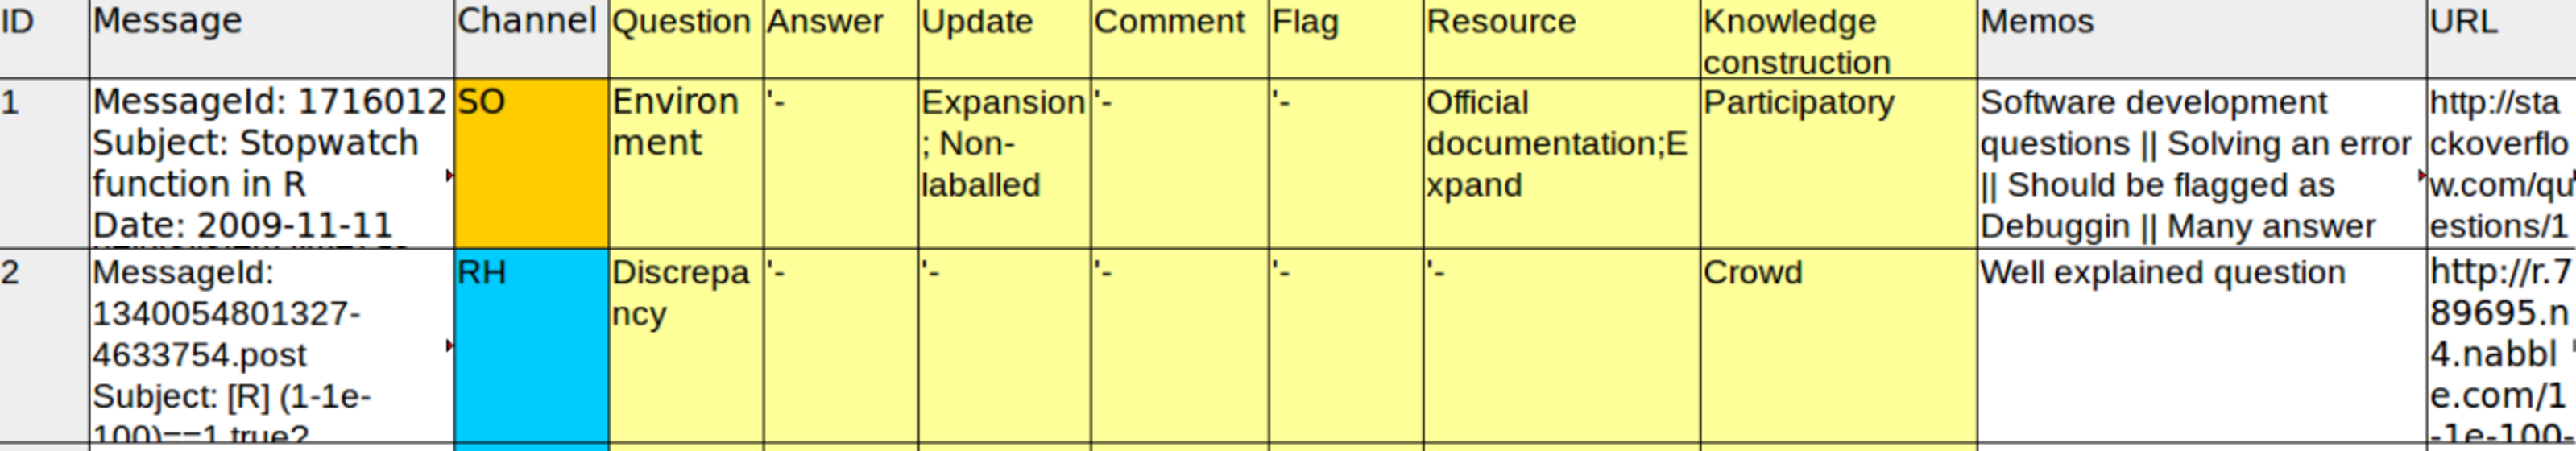
\includegraphics[width=.95\textwidth]{Figures/CodingExample}
    	\caption{Example of data coding. Each row is a thread message. Questions, comments, and answers are identified with the number on the first column. Columns in yellow contain the codification for each message type. The last two columns contain the memos and the URL.}
    	\label{fig:CodingExample}
%\vspace{-3mm}
    \end{figure*}

    \alexey{the following techniques description should be shortened. It is too much detail for a paper.}

    The techniques used to support the data analysis, which are explained as follow:

	\begin{description}[itemsep=2pt, topsep=0pt, leftmargin=1em, parsep=0pt]
		\item[Memoing] is the act of taking notes (coding) on what the researcher is learning from the data during the analysis~\cite{Groenewald2008}.
        We wrote reflective memos in a spreadsheet next to the applicable codes (see figure \ref{fig:CodingExample}).
        These memos were used to create the codes, and hypotheses about the relationships between concepts.

		\item[Affinity diagrams] allows to organize ideas and data into groups, and to find the relationships between concepts~\cite{Scupin1997}.
		We used them to discuss new insights, and while defining categories and relationships between them.

		\item[Inter-rater agreement \textit{Cohen Kappa}] is a coefficient used to measure the agreement between two coders who classify items into mutually exclusive categories~\cite{Stemler2004}.
		Ladis and Koch suggest that values above 0.60 or 60\% to obtain substantial results~\cite{Landis1977}.
		In a previous study~\cite{Gomez2013}, we used the same coefficient to measure agreement between coders.
		Based on this experience, we set a value above 0.80 or 80\% as the minimum to obtain substantial results.
		We used this coefficient after each coding session as a way to trigger discussion.

		\item[Code book] is a book that contains the definitions of the codes that researchers look during the data analysis~\cite{MacQueen1998}.
		We coded in multiple sessions, which allowed us to refine the definitions.
		Each entry is associated with a title, a formal definition, an example, and space for notes from the researcher.
		The final version of the code book is detailed in section~\ref{cha:findings}.
	\end{description}

	The focus of the analysis is to \textit{understand the context of the media channels and the community}.
	The process consisted of:
	First, a recollection of the official information for both channels and the community to build a background of the community of practice and the channels studied.
	Second, a mapping between messages from Stack Overflow with messages on the R-help mailing list.
    This is to overcome how the data is structured in both channels.
    The mapping of messages between both channels was as follows:

	\begin{description}[itemsep=3pt, topsep=2pt, leftmargin=1em, parsep=0pt]
		\item[Question:] the message is the first on the thread, and it contains the main question.
		\item[Answer:] the message provides a solution to the main question of the thread.
	 	\item[Update:] the message claims for a modification to a question (or answer) made by the author of such a question (or answer).
		\item[Comment:] the message offers a clarification to a specific part of the question or answer.
		\item[Flag:] the message requests attention from the moderator (e.g., repeated questions, spam, or rude behaviour).
	\end{description}

%	The data set was capped at 400 threads for each channel when we deemed our observations as being saturated.

\subsection{Phase 2: The survey} 

\alexey{do we use this data in any way in our paper? if not, we need either to use it or remove.}

    We conducted a survey\footnote{A copy of the survey is available at \url{http://goo.gl/mxmH5J}} with members of the R community with the purpose of obtaining additional insights on the findings.
    To test and refine the questions, format and tone, we performed two pilots.
    
    We announced our survey on Twitter, Reddit, the R-help mailing list, and Meta Stack Exchange to reach users of both channels, and minimize the selection bias.
    However, on Stack Exchange the was deemed out of topic and was deleted a few minutes later. We received 26 valid responses.

%%% Local Variables:
%%% mode: latex
%%% TeX-master: "knowledge-curation.tex"
%%% End:

% vim: set fenc=utf-8 ft=latex encoding=utf-8
% -*- mode: latex; coding: UTF-8; -*-
%!TEX root = knowledge-curation.tex
\section{Findings}
\label{cha:findings}
To understand how knowledge in the form of questions and answers is created, shared, and curated, we first identified and categorized the main types of knowledge artifacts contained in the \RH mailing list and in \SO messages with the R tag (RQ1). The emerging categories formed a typology and allowed us to identify and describe two approaches for constructing knowledge that are supported by these channels (RQ2). Interestingly, we found that some developers are active on both channels, and in some cases, even post the same questions. As a result, we investigated the benefits they gain by doing so (RQ3). In this section, we present our findings.
%This section presents the findings of our study that answer each research question.

\subsection{What Types of Knowledge Artifacts Are Shared on \SO and the \RH Mailing List}
%\subsection{RQ-1. \rqa}
\label{cha:findings-types}

To answer RQ1, we randomly sampled 400 threads of messages from both \SO and the \RH mailing list, where each thread included a question and the associated responses. We identified five main types of artifacts that capture knowledge:
\begin{enumerate*}[label=(\arabic*)]
\item Questions 
\item Answers 
\item Updates 
\item Flags
\item Comments
\end{enumerate*}
Through our analysis, we further divided these types into sub-types---table~\ref{table:type-of-knowledge} presents our typology of knowledge artifacts, their
descriptions, and their frequency in the sample of 400 threads. Even though we did not aim for a statistically significant sample size, the size of this sample
(400 threads in each channel) guarantees a confidence level of approximately 95\% $\pm$ 5\% for both channels. Using the Chi-square test of independence, we tested whether the distribution of types and sub-types of questions were different between the two channels.  In
all cases, they were found to be statistically different (with $\rho \ll 0.001$ in all cases).
    \begin{table*}[!htb]
      \centering
      \caption{Typology of knowledge artifacts found on both \SO (SO) and the \RH (RH) mailing list and their frequency in the analyzed sample. Numbers in bold represent the most significant differences between the two sets.}
      \begin{small}
\begin{tabular}[h]{p{2.3cm}p{10.3cm}rrrrr}
 && \textbf{SO}                                                                                                                                              & \textbf{RH}  & \textbf{Prop SO} & \textbf{Prop RH}                \\
\toprule
\multicolumn{2}{@{}l}{\textbf{Questions}}\\
  \emph{How-to}                   & Asks how to do something specific.                                                                                                                        & {166}          & {103}              & \textbf{41.50\% }       & \textbf{25.75\%}        \\
  \emph{Bug/Error\-/Exception}    & Asks for a solution or reasons for an error message.                                                                                                       & 27           & 48               & 6.75\%         & 12.00\%        \\
  \emph{Discrepancy}              & Asks about an unexpected result of a specific function, process, or package.                                                                              & 53           & 88               & \textbf{13.25\%}        & \textbf{22.00\%}        \\
  \emph{Set-up}                   & Asks for possible ways to set up the R environment before or after deployment.                                                                            & 15           & 31               & 3.75\%         & 7.75\%         \\
  \emph{Decision help}            & Asks for advice in making a decision.                                                                                                                     & 36           & 35               & 9.00\%         & 8.75\%         \\
  \emph{Conceptual\-/Guidance}    & Asks for conceptual clarification or guidance on topics related to R or statistics.                                                         & 48           & 49               & 12.00\%        & 12.25\%        \\
  \emph{Code reviewing}           & Asks for a code review, explicitly or implicitly.                                                                                                           & 34           & 21               & 8.50\%         & 5.25\%         \\
  \emph{Non-functional}           & Asks for help (or suggestions) with a non-functional requirement such as performance or memory usage.                                                   & 14           & 11               & 3.50\%         & 2.75\%         \\
  \emph{Future reference}         & Asks a question (often self-answering it) that might not exist on the channel, but that is interesting enough to warrant a thread for future reference.         & 5            & 4                & 1.25\%         & 1.00\%         \\
  \emph{Other}                    & Asks for assistance unrelated to the channel, or the message contains unrelated information (e.g., announcements, ideas for improvement).                  & 2            & 10               & 0.50\%         & 2.50\%         \\\cline{3-6}
                                  &                                                                                                                                                          & {400} & {400}     & {100\%} & {100\%} \\
\hline
  \multicolumn{2}{@{}l}{\textbf{Answers}}                                                                                                                                                                                                                          \\
  \emph{Redirecting}                & Provides a link to an existing solution that is not in the thread (e.g. external application, tutorial, project).                                     & 163          & 87               & 20.20\%        & 15.03\%        \\
  \emph{Tutorial}                   & Provides a set of steps to teach people how to solve the issue.                                                                                          & 105          & 15               & \textbf{13.01\%}        & \textbf{2.59\% }        \\
  \emph{Source code}                & Provides a source code snippet as the solution without an extensive explanation about the answer.                                                                   & 198          & 102              & 24.54\%        & 17.62\%        \\
  \emph{Clue/Suggestion/Hint}       & Provides a possible way(s) to fix the issue without actually solving it.                                                                                                     & 43           & 105              & \textbf{5.33\% }        & \textbf{18.13\% }       \\
  \emph{Alternative}                & Provides a different approach to a solution that is related to but not exactly what is being asked (e.g. mathematical approach, data structure modification). & 33           & 98               & \textbf{4.09\% }        & \textbf{16.93\% }       \\
  \emph{Explanation}                & Provides an explanation of an approach that answers the question and lists steps on how to do it.                                                                          & 203          & 101              & 25.15\%        & 17.44\%        \\
  \emph{Announcement}               & Provides a notification about some artifact (e.g., packages, libraries).                                                                                 & 8            & 33               & 0.99\%         & 5.70\%         \\
  \emph{Benchmark}                  & Provides a benchmark of multiple solutions posted by others or compares different answers.                                                               & 5            & 3                & 0.62\%         & 0.52\%         \\
  \emph{Opinion}                    & Provides an opinion or an expansion of another answer by including scenarios and examples.                                                                    & 49           & 35               & 6.07\%         & 6.04\%         \\\cline{3-6}
                                    &                                                                                                                                                          & \textbf{807} & \textbf{579}     & {100\%} & {100\%} \\
\hline
  \multicolumn{2}{@{}l}{\textbf{Updates}}                                                                                                                                                                                                                          \\
  \emph{Announcement}               & Announces specific events (e.g., bounties, future updates).                                                                                              & 27           & 3                & 4.40\%         & 1.21\%         \\
  \emph{Background}                 & Adds additional context to the question or answer .                                                                                                       & 74           & 57               & 12.07\%        & 23.08\%        \\
  \emph{Correction}                 & Corrects format, grammar, spelling, and semantic mistakes.                                                                                               & 301          & 2                & \textbf{49.10\% }       & \textbf{0.81\% }        \\
  \emph{Expansion}                  & Expands the question or answer by providing scenarios or examples.                                                                                       & 116          & 83               & \textbf{18.92\% }       & \textbf{33.60\%}        \\
  \emph{Explanation}                & Explains or clarifies a specific point in the question or answer, such as why the user chose a specific data structure, or the meaning of a variable.    & 83           & 95               & 13.54\%        & 38.46\%        \\
  \emph{Solution}                   & The user answers their own question.                                                                                                                     & 12           & 7                & 1.96\%         & 2.83\%         \\\cline{3-6}
                                    &                                                                                                                                                          & \textbf{613} & \textbf{247}     & {100\%} & {100\%} \\
\hline
  \multicolumn{2}{@{}l}{\textbf{Flags}}                                                                                                                                                                                                                            \\
  \emph{Off-topic/Opinion}          & Identifies questions that are unrelated to the channels' interests or which answers seek opinion.                                                      & 22           & 19               & 27.16\%        & 35.19\%        \\
  \emph{Not an answer}              & Emphasizes \textit{alternative answers} out of the scope of the question, or identifies that a solution does not answer the question.                    & 0            & 27               & \textbf{0.00\% }        & \textbf{50.00\%}        \\
  \emph{Repeated question}          & Notifies a user that the question has been answered previously.                                                                                                & 48           & 8                & \textbf{59.26\%}        & \textbf{14.81\%}        \\
  \emph{Too localized}              & Questions that are too specific and might not help future readers.                                                                                    & 6            & 0                & 7.41\%         & 0.00\%         \\
  \emph{Unclear}                    & Questions that are difficult to understand.                                                                                                              & 5            & 0                & 6.17\%         & 0.00\%         \\\cline{3-6}
                                    &                                                                                                                                                          & {81}  & {54}      & {100\%} & {100\%} \\
\hline
  \multicolumn{2}{@{}l}{\textbf{Comments}}                                                                                                                                                                                                                     \\
  \emph{Clarification}          & Provides (or requests) additional information about a question or answer.                                                                                & 98           & 28               & 17.44\%        & 10.49\%        \\
  \emph{Expansion}              & Provides additional information.                                                                                                                         & 127          & 65               & 22.60\%        & 24.34\%        \\
  \emph{Correction/Alternative} & Suggests a change to a question or answer, offers an alternative solution or a correction.                                                               & 102          & 89               & \textbf{18.15\%}        & \textbf{33.33\% }       \\
  \emph{Compliment/Critic}   & Posts something good, offers thanks, provides an opinion or criticism.                                                                           & 157          & 52               & 27.94\%        & 19.48\%        \\
  \emph{External reference}     & References an external resource.                                                                                                                         & 78           & 33               & 13.88\%        & 12.36\%        \\\cline{3-6}
                                &                                                                                                                                                          &{562}  & {267}     & {100\%} & {100\%} \\
  \bottomrule
        \end{tabular}
      \end{small}
      \label{table:type-of-knowledge}
\vspace{-3mm}
    \end{table*}

\paragraph*{Questions and Answers}
    Questions express one or more problems or concerns faced by a user on the \RH mailing list or on \SO, whereas answers represent solutions to questions.  We observed that the types of questions on \SO are more specific than those on the \RH mailing list, and \SO answers are more likely to be tutorials. Also, \SO has more answers per question---2 per question compared to 1.4 for \RH (see Table~\ref{table:type-of-knowledge}). However, \RH answers tend to offer more suggestions or alternatives than \SO answers. %This might be a result of the narrowness of \SO questions.

\paragraph*{Updates}
An update is a modification of a question or answer. In \SO, updates are presented in one of two ways.
\begin{description}[itemsep=3pt, topsep=2pt, leftmargin=1em, parsep=0pt]
\item[Labeled updates] are explicitly shown in the body of questions or answers next to a label that identifies the update (e.g., edit, update, and p.s.).
  When multiple update labels appear in a message, each label is accompanied by a number (e.g., \textit{``[Edit 1:]''}), a date (e.g., \textit{``Edit/Update (April 2011):''}), or a bulleted list
  (e.g., ``EDIT: - anova... -drop1...'').

\item[Non-labeled updates] are only visually recognizable through the message history system. The only indication of the change is a box at the end of the
  message that identifies the user who performed the change and the date when it occurred.
\end{description}
We found that \textit{non-labeled} updates are often used to correct formatting, grammar, semantic mistakes, and spelling, or to incorporate explanations, examples, and suggestions without changing the meaning of the question or answer. \textit{Labeled} updates are for everything else.

On the \RH mailing list, all communication occurs through emails, and authors do not explicitly tag messages as updates. For this reason, we define an update on \RH as \emph{a message sent to a thread where the author has already participated once}.

Regarding update frequency in our sample, the \SO R tag contained 2.5 more updates than the \RH mailing list. Corrections are more common on \SO (almost 50\%), while \RH updates are often related to the adding of information to a thread (providing background, expansion, and explanation).

\paragraph*{Flags}
Flags are used to alert members of the community that a question or answer does not match community expectations.

\SO contains a flagging mechanism, often used to get a moderator's attention. These flags can accomplish various objectives: mark a message as containing spam or rude/abusive behavior, or identify
duplicate questions, off-topic messages, unclear questions, opinion-based questions, and low-quality
answers. Depending on the type of flag, this can lead to a thread being closed or the loss of user reputation points.  

The \RH mailing list doesn't have a built-in flagging mechanism, however, \RH users utilize the concept of flags, which we define as \emph{messages used to call the attention of other community members}, similar to the way flags are used in \SO.

% The main objective of Flags in both channels is to 
% keep a
% healthy community, promote discussion, and to raise specific
% issues.  %Flags we found in emails that also contained other types of information (such as answers, comments, and updates).

% Hance, flags in the \RH mailing list do not constrain users to answer questions, or to clarify
% what it is already asked.
% Under our definition, flags might be used by the person who asked or answered a question
% (in \SO authors of a question cannot add flags to it). 

In terms of their frequency, R tag posts on \SO contained 1.5 times more flags than posts on the \RH mailing list. \SO flags are primarily used to mark repeated questions. In contrast, flags on \RH are often used to indicate that a previous answer is incorrect.

\paragraph*{Comments}

In \SO, comments are considered ``temporary `Post-It' notes left on a question or answer''\footnote{\url{http://stackoverflow.com/help/privileges/comment}}. Comments are located below each question or answer and can be used as a follow-up to a question, or to answer or clarify a question. On the \RH mailing list, we define comments as messages written to \emph{improve an answer or as a follow-up to a discussion}. It should be noted that in order for an email to qualify as a comment, it should not be written by the person who asked or answered the original question (otherwise, the message would be considered an update).
Because both \SO and the \RH mailing list permit participants to ask multiple questions in the same thread, the sub-categories of comments are not mutually exclusive.  

Regarding the frequency of comments, the main difference between the two channels is that \SO comments are less likely to be considered corrections or alternatives (Correction/Alternative sub-category) than on the \RH mailing list. The \SO R tag sample also contained 2.1 times more comments than the \RH sample (see Table~\ref{table:type-of-knowledge}).

\subsection{How Knowledge Is Constructed on \SO and the \RH Mailing List}
%\subsection{RQ-2. How is knowledge constructed on \SO and the \RH mailing list?}
\label{sec:rq2}

Our analysis helped us identify two different approaches used for constructing knowledge (RQ2) on \SO and the \RH mailing list: participatory knowledge construction and crowd knowledge construction.

\begin{description}[itemsep=2pt, topsep=0pt, leftmargin=1em, parsep=0pt]
\item[Participatory knowledge construction] is an approach where answers are created through the cooperation of multiple users in the same thread. Participants complement each other's solutions by discussing the pros and
  cons of each answer, and by adding different viewpoints, additional information, and examples.
  This process is similar to a team working together towards
  a common objective.

\item[Crowd knowledge construction] leverages the experiences of many users who work in a relatively
  independent manner. Each user contributes to the thread, adding variety to the pool of solutions. However, the user's priority is to provide a correct answer and not to discuss other solutions.
  This is comparable with the concept of a group in which people work towards the same objective but not necessarily together (e.g., Amazon's Mechanical Turk). Participants can vote on other's ideas, but the
  main idea is not constructed through a discussion process.
\end{description}

On the \RH mailing list, \textit{participatory knowledge} construction takes place when:
\begin{enumerate*}[label=(\arabic*)]
  \item previous answers are included in the current answer with clear links between them; or
  \item a reply contains a direct reference to other answers or authors.
\end{enumerate*}
Figure \ref{fig:ML-PK1} depicts two examples of the way participatory knowledge occurs on the \RH mailing list: direct citation of the author of a previous answer, and inferable links between answers.

    
    \begin{figure}[!htb]
        \centering
        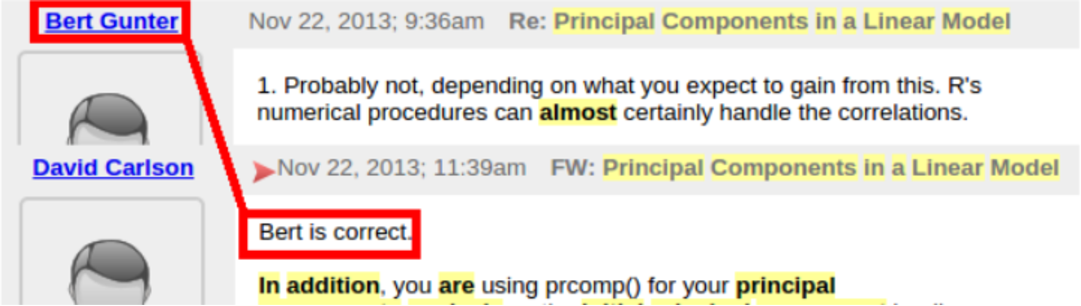
\includegraphics[width=\columnwidth]{Figures/ML-PKimg2}
        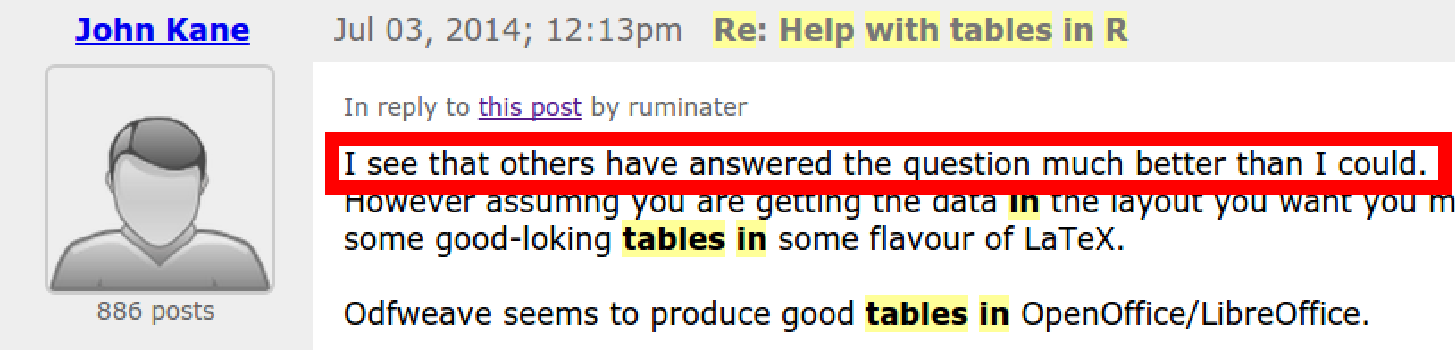
\includegraphics[width=\columnwidth]{Figures/ML-PKimg11}
        \caption[Participatory knowledge construction on the \RH mailing list.]{Participatory knowledge construction on the \RH mailing list.}
        \label{fig:ML-PK1}
      \vspace{-3mm}
    \end{figure}

On \SO, \textit{participatory knowledge} construction takes place when:
    \begin{enumerate*}[label=(\arabic*)]
    \item one can infer a link between answers, through either a direct or indirect reference; or
    \item comments complement the answer or directly cite another author.
    \end{enumerate*}
Participatory knowledge construction also occurs in different places on \SO, perhaps as a consequence of its rich interface. We observe this type of knowledge construction when a user answers a question and directly cites or links to someone else's answer in the thread, or when a user cites someone else's question or answer in a comment (a typical case is linking to a previously asked question). Figure \ref{fig:SO-PK1} depicts an example of participatory knowledge construction on \SO: when an answer was deemed insufficient, a user helped out by adding a comment and referencing another author's answer.

    \begin{figure}[!htb]
        \centering
        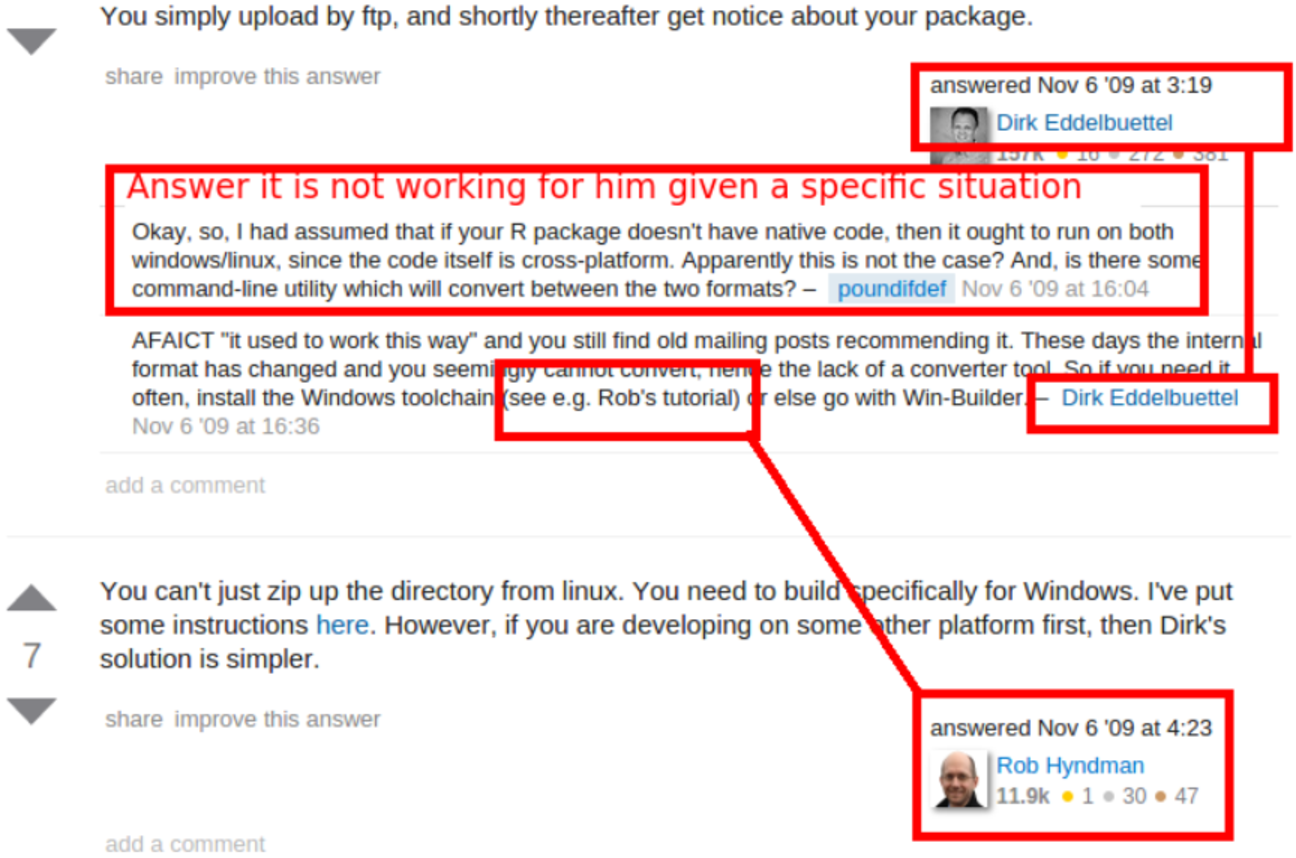
\includegraphics[width=\columnwidth]{Figures/SO-PKimg5}
        \caption{Example of participatory knowledge on \SO. Users built on the comments and answers of other users.}
        \label{fig:SO-PK1}
        \vspace{-3mm}
    \end{figure}

On \SO, \textit{crowd knowledge} construction is observable when:
  \begin{enumerate*}[label=(\arabic*)]
    \item there is no direct or inferable reference between answers; or
    \item an answer is a variation of one of the other answers on the thread.
  \end{enumerate*}
Figure \ref{fig:CKC_MLSO} depicts an example of crowd knowledge construction on \SO. As can be seen from the figure, two of the three answers provided the same solution. 

On the \RH mailing list, we observed \textit{crowd knowledge} construction when different messages responded directly to the original question, rather than to another response.

    \begin{figure} [!htb]
        \centering
        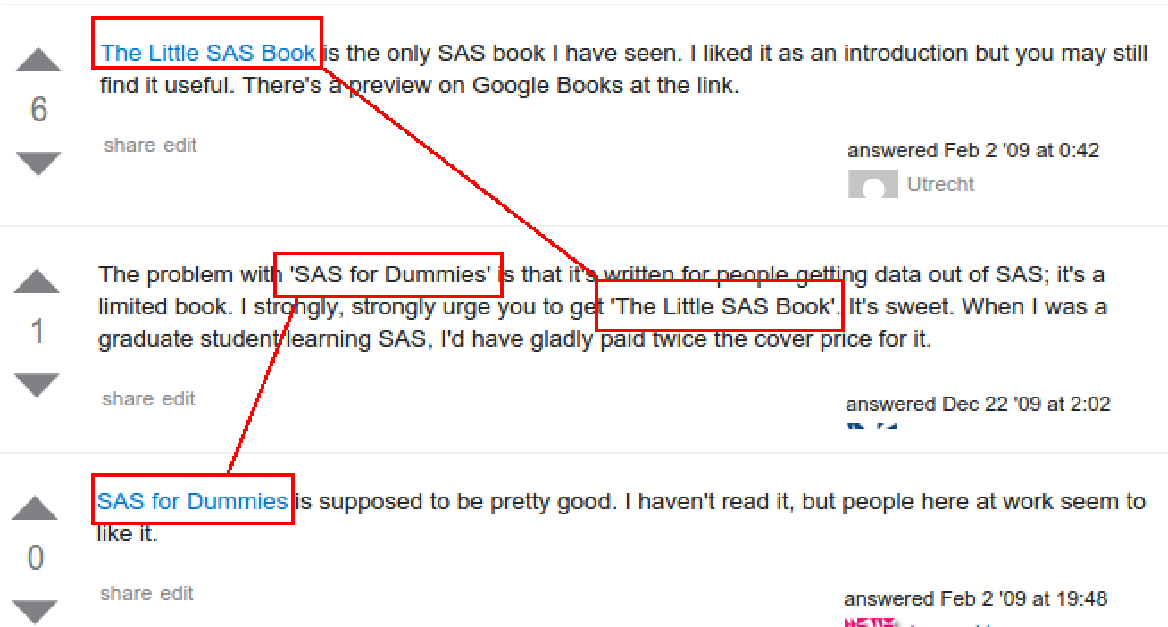
\includegraphics[width=\columnwidth]{Figures/SO-CSimg2}
        \caption{Example of how crowd knowledge construction occurs. The three authors provided similar answers, but did it independently of each other.}
        \label{fig:CKC_MLSO}
\vspace{-3mm}
    \end{figure}

\subsection{Why Users Post to a Particular Channel}
%\subsection{RQ-3. Why do certain users post to both \SO and the \RH mailing list}
From our survey, we were able to learn why some R community members preferred one channel over the other. We summarize their responses below.

\subsubsection{Why Participants Post on \SO}

Survey participants preferred using \SO for several reasons: (a) the ability to gain peer recognition (the advantage of gaining points---and visibility---is a major draw of \SO); (b) its rich and user-friendly interface; (c) answers are straight to the point; (d) questions are usually answered faster on \SO than on the \RH mailing list; and (e) it is easy to search for previous questions and answers.

However, the respondents reported a few main drawbacks of using \SO: (a) there is an overabundance of related questions; (b) one requires a certain level of experience to understand some of the answers; and (c) \SO's strict rules only allow questions and their answers, they do not allow discussions nor questions about opinions.


\subsubsection{Why Participants Post on the \RH mailing list}
\label{sec:rh}

Survey participants reported a few benefits of using the \RH mailing list: (a) the email format is convenient; (b) following the mailing list provides awareness and increases learning in new topics; (c) there is more flexibility regarding the topics that one can discuss; and (d) there is much participation from highly experienced users. The respondents did note a couple of disadvantages of \RH: (a) some discussions lead to aggressive behavior; and (b) searching the archives is not easy.

\subsubsection{Why Participants Post to Both Channels}

Our analysis of the archived data revealed that some users (79 cases in our sample) posted the same question on both channels. 
%The survey provided deeper insights on why R members act this way.
Based on the responses from the survey, we identified that being active on both channels brings benefits to those asking and answering questions (RQ3).

\begin{description}[itemsep=2pt, topsep=0pt, leftmargin=1em, parsep=0pt]
\item[Find a better answer:] As expected, two channels are better than one as 
  one channel might result in a better answer than the other.
\item[Support follow-up questions:] We found that the \RH mailing list is often used to conduct follow-up discussions on
  specific answers provided to \SO questions. \SO's focus is on finding an answer to a question and does not
  provide an environment to discuss the specifics of an answer (unless it is asked as another question).
In contrast, a discussion on \RH can continue long after an answer has been found through follow-up questions, and not only by the person who asked the original question.  
\item[Speed up answers:] Members ask the same question on both channels in order to get an answer faster. However, this behavior is not encouraged by the community as it is deemed impolite\footnote{\href{https://goo.gl/p9vVaj}{https://goo.gl/p9vVaj}}.
% `... it's impolite to cross post across several lists (i.e., \SO and \RH)''
\end{description}





%%% Local Variables:
%%% mode: latex
%%% TeX-master: "knowledge-curation.tex"
%%% End:

% vim: set fenc=utf-8 ft=latex encoding=utf-8
% -*- mode: latex; coding: UTF-8; -*-
%!TEX root = knowledge-curation.tex

\section{Discussion}
\label{cha:theory}

In this section, we reflect on the results presented in the previous section and place them within the context of related research. Additionally, we identify research opportunities and derive recommendations for using multiple Q\&A channels.
In the following, we provide representative quotes extracted from the survey, using P\# to indicate the participant ID.

\subsection{Knowledge Creation and Curation}

    Based on the results, both channels seem to provide roughly the same knowledge support for questions and answers.
    However, there are some important differences between the channels, which are summarized in Table~\ref{table:constrat}. We discuss each in detail below.
%    These observations are tendencies, and they are not behaviours unique of each channel.

    \begin{table}[!htb]
      \centering
      \caption{Comparison of the way knowledge is shared on \SO and the \RH mailing list.}
      \label{table:constrat}
      \begin{small}
        \setlength{\tabcolsep}{5pt}
        \begin{tabular}{@{}lll@{}}
          \toprule
          \textbf{}      & \textbf{\SO} & \textbf{\RH}\\
          \midrule
          Knowledge construction & Mainly crowd             & Mainly participatory \\
          Topic restriction      & Yes & No \\
          Emphasis & Curating knowledge & Developing knowledge \\ 
          \bottomrule
        \end{tabular}
      \end{small}
\vspace{-3mm}
    \end{table}

\subsubsection{Knowledge construction}

\SO's gamification mechanism encourages users to be first when answering questions~\cite{Singer2013}. In contrast, the \RH mailing list is a less competitive
environment, where users tend to build on other responses. In \RH, users work as a team, rather than as individuals searching for points (as is the case on \SO).
As a result, knowledge on \SO is built in a more crowdsourced manner, while knowledge on the \RH mailing list is usually built in a participatory manner.

The competitive \SO environment creates an incentive to be the first to answer, rather than improving and building on other answers. It's not uncommon to find a question with several answers that provide the same information. For example, three of the six answers in the \SO question titled \textit{``Resources for learning SAS if you are already familiar with R''}\footnote{\url{http://goo.gl/Mb4Pbk}} referenced the same books.
%    The gamification mechanism gives reputation to those who answer the questions, even when each extra answer might not add any new insight about how to solve a specific problem.
And while \SO provides a powerful curation mechanism to ensure the best answers make it to the top, it does not explain why an answer is better than another.

In contrast, the \RH mailing list tends to be more participatory in how users construct knowledge and it fosters an environment where users discuss proposed answers. Its users tend to provide more background to the answers and explain the rationale behind them.

For example, the question \textit{``Arrange elements on a matrix according to rowSums + short `apply' Q''} was posted to both \SO\footnote{\url{http://goo.gl/a8AES8}} and {\RH}\footnote{\url{http://goo.gl/PGflT5}}. This question illustrates the contrast in how the two communities build knowledge.
On \SO, each participant contributed a solution without any evidence of collaboration with others.
Whereas users on the \RH mailing list complemented each other's answers by providing further information and insights to the answers already
contributed. Vasilescu \textit{et al.}~\cite{Vasilescu2014c} showed that members who are active in both channels tend to provide answers faster on \SO than on \RH,
suggesting that they are motivated by the gamification aspects of \SO, and thus they tend to gravitate towards crowd knowledge construction.

    
While prevalent, the construction of knowledge on \SO is not limited to the crowd-based approach. Participatory knowledge construction is also existent, such as by up/down voting questions and providing comments. In most cases, participatory knowledge construction on \SO is used for editing answers (e.g., correcting grammar) or linking to previously asked questions.
Similarly, some knowledge on the \RH mailing list is constructed in a crowd-based manner, but this form is less prevalent than the participatory one.

Tausczik \textit{et al}.~\cite{Tausczik2014} examined how members of Math Overflow (a Q\&A platform for mathematicians) collaborate and construct knowledge. They found that collaboration was diverse and fell on the spectrum between \textit{independent} (crowd-based) and \textit{interdependent} (participatory). Similar to our findings with \SO, the most common collaborative act was of an independent nature (i.e., providing information), while other contributions that built on existing work were less common (i.e., clarifying the question, critiquing answers, revising answers, and extending answers).

Our results seem to imply that \SO's gamification features, while highly effective, have the side effect of reducing collaborative knowledge creation between users. In their study on building \SO reputation, Bosu \textit{et al.}~\cite{Bosu2013} proposed six strategies for increasing reputation score, two of which were: be the first to answer, and do it at \textit{off-peak hours}---indicating crowd knowledge creation. Furthermore, while \SO gives people the ability to vote on comments, it does not reward points to users that post comments. For example, some users search \SO for answers within comments and convert them to proper answers to gain reputation points\footnote{\url{http://duncanlock.net/blog/2013/06/14/the-smart-guide-to-stack-overflow-zero-to-hero}}.


    % The findings presented here as theory can be used to identify how channels' features or community members might affect the construction of knowledge.
    % For instance, we identified that gamification might affect collaboration between users. 
    % Users prefer to create their own answer instead of collaborating with others.
    % Additionally, it might be possible for indirect collaboration, like the one happening on the comments on \SO to improve discussion and participatory knowledge construction if there was a mechanism to provide points for this type of participation.
%    However, more studies are required to extend our observation to other domains, communities, and channels.

\subsubsection{Topic restriction}

\SO's participation rules only permit questions that have a clear answer, making it topic restrictive. In contrast, the \RH mailing list is suitable for discussing
any topic related to the R language. For example, questions related to R but not focused on software development are not rejected by the \RH mailing list community---topics that trigger discussion are welcomed!
%    For instance, when users discuss the creation or improvement of the R community channels (see section \ref{sec:userbeh}); or when a question about installing R on \textit{Linux} is asked on the \RH mailing list (like {\href{http://goo.gl/1JLOUF}{\textit{``R on X11 under Linux''}}}).

\SO questions that trigger a discussion are flagged as opinion-based or off-topic and will likely be closed. Correa and Sureka~\cite{Correa2014} found that 18\% of deleted questions on \SO are subjective (i.e., ask for opinion).
For example, a question titled \textit{``What's a good example of really clean and clear [R] code, for pedagogical purposes?''}\footnote{http://goo.gl/9JjZW1} was flagged as \textit{off-topic} because the question was not related to software development.
An \RH user wrote a fine explanation of the purpose of each channel in a message on the mailing list:\footnote{\url{http://goo.gl/mTccwx}}:
    \begin{quote}
        \textit{``Got an R programming question that you think has a definite answer? Post to [\SO]. Want to ask something for discussion, like what options there are for doing XYZ in R, or why lm() is faster than glm(), or why are these two numbers not equal? Post to \RH. Questions like that do get posted to [\SO], but we [vote] them down for being off topic and they disappear pretty quickly.''}
    \end{quote}

Squire reported that, despite the gains in participation and the response time provided by \SO, many development communities keep using mailing lists, either as
a primary communication channel or as part of a hybrid solution where multiple channels are used, thus allowing for non-restrictive topics and fostering of
discussion~\cite{Squire2015a}.
Mailing lists are also favored for their simplicity, and for allowing guaranteed delivery (i.e., knowing who will receive the email) ~\cite{Zhang2015}.

    % We believe it is important to understand how the knowledge is constructed on media different channels, and how different mechanisms such as gamification or topic restriction can affect the knowledge construction~\cite{Li2015}.
    % Through this understanding, researchers can gain insights of how to support future media channels, and user diversity~\cite{Vasilescu2014b}.

\subsubsection{Curated knowledge and knowledge development}

One of the main benefits enabled by \SO's crowd-based knowledge construction is the creation and curation of a pool of questions and answers. In contrast, \RH provides an environment in which users
    develop knowledge through participation, but this knowledge is not curated for future use. This makes the information difficult to be reused by those who were not
    participants (either active or passive) during its creation.


    % On the \RH mailing list questions tend to have more background than on \SO.
    % The knowledge embedded in the \RH mailing list's answers can be used to learn new procedures, as well as identify the train of thought that guided
    % participants when forming an answe
While \SO has been successful, some users feel that by not fostering discussion, it restricts thinking that might lead to better answers, as P26 explained:
    \begin{quote}
        \textit{``Many developers share my view that [\SO] is a very bad model, ... [it] removes the value added by reading list traffic that doesn't seem directly relevant to a currently conceptualized question, but which may lead to a new conceptualization (out-of-the-frame thinking). [\SO] cannot do that.''}
    \end{quote}
    Similarly, P35 stated that they use the \RH mailing list if the questions are not 100\% \textit{``help-me-to-code-this''}.

    However, \SO shines when questions have to be kept for posterity. 
    Its curation mechanisms provide tools for keeping the channel clean of what seems to be unnecessary information (e.g., flagging questions, deleting comments, editing messages, and demoting irrelevant answers), as P14 explained:

    \begin{quote}
        \textit{``[\SO] is an excellent model for providing a rich resource for users of R, which the \RH mailing list was not. 
        Ability to include light markup, render code blocks nicely, no nested email threads all helps the experience of searching for and finding the help that a user needs, and I want to contribute to that.''}
    \end{quote}

    % Thus, we identified that there are certain benefits for keeping the history of the question available.
    % As U26 said, there are some benefits to reading what a user thinks is not important for conceptualized questions, but which may lead to out of the frame thinking. 

\subsubsection{Research opportunities}

An important research question that arises from these findings is whether \SO's model can be improved to provide better participatory knowledge construction support without hindering its ability to curate information for future use.

Another interesting aspect emerging from our findings is that the activity on the \RH mailing list is only marginally smaller than on \SO (the proportion of responses in each category fluctuated between 1.4 and 2 times). Further research is required to verify the quality and effectiveness of answers.

\subsection{Recommendations for Using Multiple Q\&A \Channels}

    \begin{table*}[htbp]
      \caption{Recommendations to improve the benefits from using several Q\&A channels.}
      \centering
\small
      \begin{tabularx}{1.0\linewidth}[h]{@{}p{4.6cm}X@{}}
          \toprule
\reca & Make sure the channel is the best according to the nature of the question.\\
\recb & Make sure the question uses proper nomenclature and does not violate the rules of the channel.\\
\recc & Explain the context that prompts one to ask such a question.\\
\recd & Reference external resources appropriately and use tools (such as gists.github.com) that enable others to help .\\
\rece & Help others and work towards improving the community and the channels.\\
          \bottomrule
      \end{tabularx}
      \label{tab:recom}
\vspace{-3mm}
    \end{table*}

One of the expected outcomes of this study is a set of recommendations for using multiple \channels. Based on existing literature and our results, we provide five recommendations for people seeking or contributing answers.  Our recommendations are summarized in Table~\ref{tab:recom}.

%Overall, both channels complement each other and the R-community benefits from using both

%     By studying communities that migrated development support towards \SO, Squire~\cite{Squire2015a} found that the main reason for communities coming back to the mailing list is topic restriction and the question format expected on \SO.
%     Our findings supports Squire's suggestion that communities of practice evaluate the real benefits of each channel before moving to newer technologies.






\subsubsection{\reca}


    Each channel provides a list of \textit{topics} that are deemed acceptable.
    The topics are regulated either by the community or the channel's moderators. \textit{``...\SO has (a) more limited range of help topics (help for code only), whereas \RH is broader (philosophy, posting announcements, etc.)''} [P35].
    Knowing which channel is more suitable for a specific topic can improve the response time or the quality of the answer.

%\dmg{The following is not clear and I would delete it}
%    Additionally, \textbf{choosing the proper channel keeps the knowledge where it is most useful, thus enhancing the quality of the content of the channel}.
%    For example, in the \RH's thread \textit{``Bumps chart in R''}\footnote{\url{http://goo.gl/EJHWrs}}, a user wrote: \textit{``(cross posting to the ggplot2 group for posterity) Here's how I'd approach it...''}, that is, cross-posting the question---previously posted and answered on the \RH list---in order to keep a record of the knowledge where it reaches more users, and where it is more useful to the community.

    In some cases, it is expected that questions will be answered by a \textit{specific group} (e.g., R-core team) regardless of the topic, as P32 stated: \textit{``If I really want an answer from someone in R-core or closely related people, I would definitely choose the mailing list''}.
    For example, in the \RH thread \textit{``Co-integration and ECM in Package \{urca\}''}\footnote{\url{http://goo.gl/7olLv7}}, a participant asked the R-core team how to solve a problem: 
     \begin{quote}
     \textit{``Dear R Core Team, I am using package \{urca\} to do co-integration and estimate ECM model, but I have the following two problems...''}
     \end{quote}
    In this scenario, Websites associated with a specific package or library might be the best way to communicate directly with the creators of that technology. Thus, \RH is a place for discussion and \SO is a place for questions that have a clear answer.

     

%\dmg{I do not understand the following}
%In some cases, the description of the channel or package provides the necessary information, such as the maintainers or participants (e.g., \RH primary help webpage\footnote{\url{https://stat.ethz.ch/mailman/listinfo/\RH}}, \emph{rcpp} package\footnote{\url{https://cran.r-project.org/web/packages/Rcpp/index.html}}, or \textit{r-tag} info page on \SO\footnote{\url{http://stackoverflow.com/tags/r/info}}).
%    Figure \ref{fig:CCchannel} depicts an example of how developers of a package can be reached using \SO (on the left) or by email (on the right). 

%    \begin{figure} [!htb]
%        \centering
%        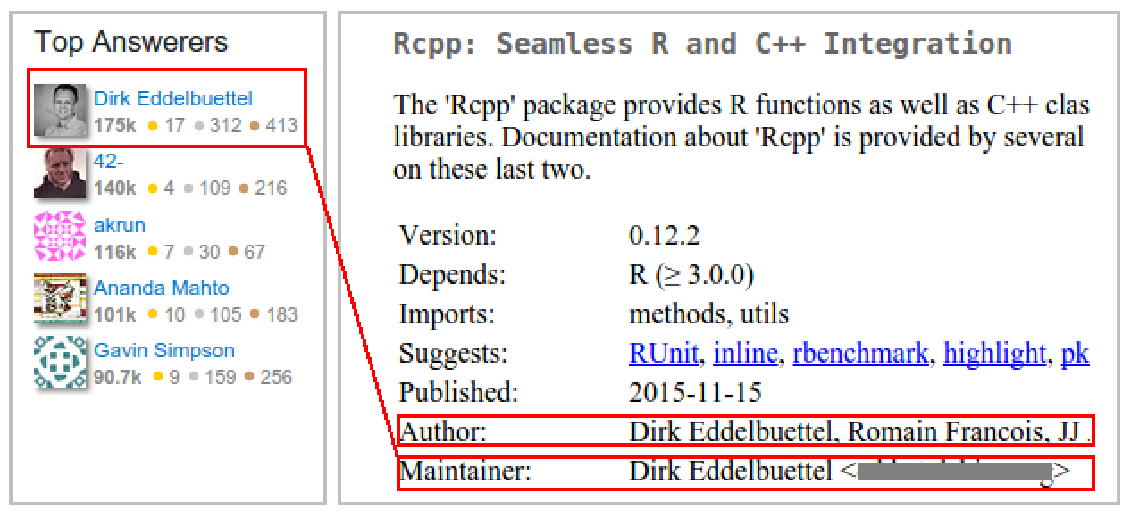
\includegraphics[width=\columnwidth]{Figures/CCchannel}
%        \caption{Example of how to reach developers of the \emph{rcpp} package. On the left, \SO, and on the right, the \emph{rcpp} webiste.}
%        \label{fig:CCchannel}
%    \end{figure}

%    Some channels are more suitable for certain \emph{type or format of questions}. 


\subsubsection{\recb}

    Throughout this study, we noticed that most of the harsh responses were given to users who did not learn the participation rules or had not learned the basic concept of R or statistics.
    For anybody using a channel, the community expects users to familiarize themselves with the channel in advance and learn the basics of the technology that they are discussing.

    % For instance, in the \RH's thread \textit{\href{http://goo.gl/Dc8gXw}{``Quantile''}} it is remarked the points of a guide that the user asking the question did not follow: \textit{``...Please read the Posting Guide. It asks that you not crosspost. If you post a followup to rhelp, then the reading of the Posting guide will tell you that much more in the way of detail about your setup was requested...''}.

%    Depending on the channel, the amount of guide lines and posting guides available might differ. 
    \SO provides user guides\footnote{\url{http://stackoverflow.com/help}} for each of the main features of the channel, such as badges, questions,
    answers, flags, comments, and the reputation system. While, the \RH mailing list only has general instructions\footnote{\url{https://www.r-project.org/mail.html\#instructions}} and a guide about posting on the channel\footnote{\url{https://www.r-project.org/posting-guide.html}}.

We also discovered that the R community has developed resources to improve the quality of participation on the communication channels.
%    Moreover, depending on the purposes of the \channels, there might exist community-developed guide that should be read before participating in the channel.
    For example, the post on \SO \textit{``How to make a great R reproducible example?''}\footnote{\href{http://stackoverflow.com/questions/5963269/how-to-make-a-great-r-reproducible-example}{http://stackoverflow.com/questions/5963269/how-to-make-a-great-r-reproducible-example}} provides tips and tricks for creating a reproducible example using the R language.
    Another example is the document \emph{How to write a reproducible
      example}\footnote{\url{http://adv-r.had.co.nz/Reproducibility.html}}, which provides tips for posting a reproducible R code example to mailing lists: \textit{``...Before putting all of your code in an email, consider putting it on \url{http://gist.github.com/}{[GitHub Gist app]}. It will give your code nice syntax highlighting, and you don't have to worry about anything getting mangled by the email system...''}

    Finally, there are manuals like \textit{``An Introduction to R''}, and the FAQ Webpages for R that are available to the public---most of the time, free of charge---and from which any user can learn the basics of R.
    For example, the R community provides a compendium of PDF documents for new users of different languages\footnote{The R manuals are available at \url{https://cran.r-project.org/}}.
    In \SO, supported technologies are provisioned with Webpages and links to free and paid materials\footnote{Materials available at \url{http://stackoverflow.com/tags/r/info}}.
    %Members are able to reference these materials when needed, e.g., \textit{``...You may want to acquaint yourself with the 'An Introduction to R' manual that came with your R installation to learn more about indexing.''}



\subsubsection{\recc}

    In spite of reading the documentation, a user may fail to address the channel appropriately.
    The community may feel that the question asked, the information provided, or something else entirely is not in compliance with the expectations and rules of the channel.
    In such cases, one should describe the documentation read, the attempts made, and the goal(s) they want to achieve.
    This would avoid answers like \textit{``read the manual''} or \textit{``read the posting guide''}. %, as well as helping the participants to help.
    For example, in the thread \textit{``lme4 GLMM''}\footnote{\url{https://goo.gl/Gbek3R}}, the user explicitly acknowledged the repeated question and explained the rationale for doing so: \textit{``I'm very sorry for my repeated question, which I asked 2 weeks ago, namely: I'm interested in possibly simple random-part specification in the call...''}.


\subsubsection{\recd}

    A common practice to answer or ask questions is to provide links for documentation, examples, source code, or other resources.
    As links point to online resources that might not exist in the future, it is important to include the key points of the resource within the question or answer.
    For instance, when a question or answer contains information in an external file hosting service like Dropbox or Google Drive, the owner of the service account can remove or break the link at any moment, leaving the message incomplete or impossible to reproduce. %An example can be seen in the thread\textit{\href{http://goo.gl/5nanFU}: {``Is it possible to create a 3D contour plot without continuous data in R?''}}.
    P33 suggested that \textit{``Questions should be self-contained as much as possible. Exceptions: recognizable links such as CRAN, R documentation, etc.''}.

    Based on our observations, we provide the following set of recommendations for using third-party resources within links.

    \begin{description}[itemsep=3pt, topsep=2pt, leftmargin=1em, parsep=0pt]
        \item[Use well-maintained Websites] that are expected to be available in the future, such as Wikipedia and the official documentation in CRAN.
        For example, %in the \SO thread \textit{``calculating convolution of multinomial distribution''},
        a user on \SO posted: \textit{``I'm doing a simulation where I need to calculate a \href{https://en.wikipedia.org/wiki/Convolution_of_probability_distributions}{[Wikipedia link] convolution} of
          \href{https://en.wikipedia.org/wiki/Multinomial_distribution}{[Wikipedia link] multinomial distributions}...''}.

        \item[Use resources that support or expand the message] to further clarify the message for those who might need it. For instance, a thread on \SO titled \textit{``How do I save all the draws from a MCMC posterior distribution to a file in R''} states \textit{``...You should be able to open a text connection using ?file \href{http://stat.ethz.ch/R-manual/R-devel/library/base/html/connections.html}{[more information]} with the open argument set to write...''}.

        \item[What to do when material relevant to the message is too big.] It is not always practical to include all the related information in a message. In this
          case, a link might be a better alternative, such as referencing videos or documents as links rather than including them as attachments.
        For example, in the \RH thread \textit{``Using FUNCTION to create usable objects''}, a user linked to a PDF rather than quoting it: \textit{``I suspect you are trying to find your way
          into Circle 6 of `The R Inferno' but haven't yet got in. \href{http://www.burns-stat.com/pages/Tutor/R\_inferno.pdf}{[link to PDF of R Inferno]}''}.
    \end{description}

\subsubsection{\rece}
\label{sec:userbeh}

It is obvious that users help others by answering questions. However, while analyzing questions and answers, we identified positive user behaviours that
we believe are worth mentioning.  These behaviours provide evidence of an altruistic way of thinking and the strong commitment that users have towards building knowledge in their community.

\begin{description}[itemsep=2pt, topsep=0pt, leftmargin=1em, parsep=0pt]
\item[I answered my own question:] Some questions are answered by the user that asked the question. They posted back to the channel to document their solution and help others: \textit{``Just for the records (and if anyone ever wants to find the `solution'), I solved my own problem.''}\footnote{\url{https://goo.gl/r3z0DX}}. 
 
\item[I did it for you:] When answering, authors provide source code to help others: \textit{``I coded up the algorithm from the Cameron and Turner paper. Dunno if it gives exactly the same results as my (Splus?) code from lo these many years ago...''}\footnote{\url{http://goo.gl/GXWGG3}}.

\item[Updated or continued years later:] Some questions are answered months or years later.
For example, a user on \SO modified an answer to provide a more updated version of the source code\footnote{\url{http://goo.gl/k6ZARR}}, and a {question asked on the \RH mailing list in 2012 was continued two years later}\footnote{\url{http://goo.gl/kgSHZv}}.

\item[Ideas to improve the channel:] This behaviour is specific to the \RH mailing list. Sometimes users suggest modifications or new features to improve the channel. For example, a {user proposed to create a package repository that can be accessible through a public wiki or version control interface}\footnote{\url{http://goo.gl/p0IunD}}.
\end{description}

% \dmg{I would remove the two following bullets:}

%     We also identified 2 behaviours that might result in a negative response from the community:
%     \begin{packed_enum}
%         \item \textbf{Cross-posting:} The user posts the same question in both channels at the same time.
%         For instance: \textit{\href{http://goo.gl/ENKrVK}{``-1 for cross posting to \RH – [user name]''}}.
% \dmg{This needs an example of a bad response, not just a crossposting, since this example does not show why users dislike it}
% \dmg{This next one sounds repetitive... it is already above in learn to use the chnanel}
%         \item \textbf{Posting guidelines violation:} The user behaves in a way that it becomes apparent that they did not read the posting guidelines.
%         For instance, a user asked a question that seems to be the opposite of what the posting guide recommend, and someone answered: \textit{\href{http://goo.gl/FUm1HC}{``...If you read the Posting Guide I think you will find precisely the opposite expectation explicitly presented. Using my "cheeky code" would only be part of the recommended actions to take before posting if you follow the recommendations of the "Do your homework before posting:"...''}}.
%     \end{packed_enum}

%\dmg{This section needs a way to finish}


\subsection{Threats to Validity}
\label{cha:threats}
Here we examine and discuss threats to the validity of our approach~\cite{Runeson2012}.
%\dmg{This is a section that can be shorten as needed in case of space issues... but first we need to finish the sections before }

%\remarks{Consider making the data available online.}
\begin{description}[itemsep=3pt, topsep=2pt, leftmargin=1em, parsep=0pt]

\item[Construct validity:] to reach the emerging themes, we rely on subjective human judgment during the data coding phase. Researchers had to decide if a message falls within a specific coding category. To alleviate this issue, two researchers coded the qualitative data as part of the analysis process. We applied the Cohen Kappa coefficient on categories that were not mutually exclusive, whose purpose was to trigger discussion between coders. We set a threshold of 0.8 as the minimum to obtain agreeable results, which is higher than the 0.6 suggested in the literature~\cite{Landis1977}.
%To minimize this threat, we used multiple data sources to triangulate our findings (survey, documentation, and messages from two different \channels), we randomly selected data, and two researchers performed the data coding.  

\item[Internal validity:] \SO's data is structured while \RH consists of unstructured data. As a result some of the mapping between both channels was straightforward (e.g., a follow-up to a reply is a comment to that question), while in other cases it wasn't as obvious (e.g., identifying some emails as questions). To reduce risk of bias when mapping the messages between both channels, two researchers performed the mapping.  


% in order to compare the emails to the \SO discussions we had to map the types of messages from one channel to the
% other. The \RH mailing list is unstructured emails that are connected between each other when they belong to the same thread. In contrast, \SO has a rich
% data type (questions, answers, comments, flags, etc.). Some of this mapping is automatic: a reply is a response to the original question, a follow-up to a reply
% is a comment to that question. Other had to be done by hand, this includes identifying some emails as containing a question, or a being a ``flag''.
% Also, \SO is newer than \RH, and for that reason we only used messages from \RH that were created after \SO was created.
% Two researchers performed this mapping to reduce any bias that it might have  introduced.

% Additionally, our understanding of that data and the observations we made played a big role in the mapping exercise, and it is subject to research bias.  To
% minimized the bias, two researches performed the mapping.

\item[External validity:] our case study is exploratory in nature and we purposefully aimed to study the R community. Many R users are likely to be \textit{casual developers} with limited or non-existent programming experience, and with backgrounds that vary from biologists to statisticians. Thus our findings may not apply to other developer communities. However, since \SO and mailing lists are widely used by other communities, we believe that our findings may be extended to these communities as well~\cite{Squire2015a}. We do not claim the generalazability of our findings to other communication channels (e.g., Slack, GitHub), and further research is required to examine how knowledge is shared on other channels used by developers.

% This type of case study cannot be assumed to be generalizable until further evaluations have been conducted~\cite{Yin2009}.
%     Hence, the findings of this research should be tested in other communities and with other channels to see if they apply to these other contexts.
% Another aspect to consider is that the R-community might not be composed of traditional programmers.
%     The R programming language is used to solve statistical problems, where the product is the statistical analysis or graphs it creates. The scripts written in
%     R are not the product, but the means to a product.
%     Also, many R language users are likely to be \textit{casual developers} with limited or non-existent programming experience, with backgrounds that vary from
%     biologists to statisticians. As a consequence, this study might not represent the knowledge that a software developer community shares. 
\end{description}

%%% Local Variables:
%%% mode: latex
%%% TeX-master: "knowledge-curation.tex"
%%% End:

% vim: set fenc=utf-8 ft=latex encoding=utf-8
% -*- mode: latex; coding: UTF-8; -*-
%!TEX root = knowledge-curation.tex
\section{Conclusions}
\label{cha:conclusion}

    Understanding the interplay between channels should be the next step to gain further insights into software development practices.
    To that end, we contrasted the way knowledge is shared on Stack Overflow and the R-help mailing list, as well as an extensible categorization of Q\&A channel messages that is meant to be used to compare and analyse knowledge in media channels.
    To conduct a fair comparison, we collected raw data from both channels, transformed this data to a common format through an analysis of the messages to map questions, answers, and other elements.

    After the analysis of more than 500 threads, we identified five types of messages: question, answer, comment, update, and flag; and more than 35 categories along with their properties, including how-to question, tutorial answer, announcement update, not-an-answer flag, and clarifications comment.

    We identified two mechanisms for the construction of knowledge: \emph{participatory}, in which answers are created with the collaboration of various users; and \emph{crowd-based}, which is non-collaborative and where solutions are posted without any acknowledgement to previous answers.
    We also analysed links and how these contribute to the construction of knowledge, such as by referencing source code, projects, and other posts related to a particular question.

    We also identified user behaviours based on their comments.
    We noted certain usage characteristics such as solving their own question by providing the answer, and cross-posting in both channels.

    To bring further insights on our findings, we conducted a survey that collected 26 answers from R users.
    The result was a list of pros and cons of using both channels. We incorporated them in the set of recommendations for using multiple channels and resources.

%%% Local Variables:
%%% mode: latex
%%% TeX-master: "knowledge-curation.tex"
%%% End:


\bibliographystyle{abbrv}
\bibliography{references}

\end{document}

%%% Local Variables:
%%% mode: latex
%%% TeX-master: t
%%% End:
